\documentclass[3p,twocolumn]{elsarticle}

\usepackage{hyperref}
\usepackage{amsmath}
\usepackage{booktabs}
\usepackage{graphicx}
\usepackage{listings}

\journal{SoftwareX}

\begin{document}

\begin{frontmatter}

\title{HydroSmart-MA: An open-source, satellite-driven decision support system for precision irrigation in water-scarce regions of Morocco}

\author[aff1]{Ayoub Admin\corref{mycorrespondingauthor}}
\cortext[mycorrespondingauthor]{Corresponding author}
\email{ayoub.admin@student.ma}

\author[aff1]{Co-Author Name}
\author[aff1]{Academic Advisor}

\address[aff1]{Department of Precision Agriculture and Digital Development, Souss-Massa University, Agadir, Morocco}

\begin{abstract}
Morocco is experiencing an unprecedented water stress crisis, with groundwater depletion rates in agricultural basins like Souss-Massa exceeding sustainable recharges by over 300 million cubic meters annually. Traditional irrigation scheduling relies on subjective human intuition or rigid, calendar-based intervals, leading to severe water waste or crop stress. To address this challenge, we introduce HydroSmart-MA, an open-source, multi-platform decision support software suite designed to compute crop-specific, high-precision irrigation scheduling in real-time. The platform consists of a Next.js administrative web dashboard and a Flutter mobile application for smallholder farmers, connected through a unified Supabase cloud database. HydroSmart-MA calculates daily reference evapotranspiration ($ET_0$) using the FAO-56 Penman-Monteith equation driven by real-time local weather API coordinates. To solve the problem of field-specific, dynamic crop coefficient ($K_c$) estimation, the software integrates live Sentinel-2 satellite imagery via the Agro Monitoring API, converting Normalized Difference Vegetation Index (NDVI) measurements into daily crop water needs. Furthermore, it models daily root zone soil water depletion ($D_r$) to trigger irrigation recommendations only when the readily available water ($RAW$) is depleted. This paper describes the software's architecture, key functionalities, mathematical models, illustrative Moroccan crop scenarios, and its educational and economic impacts.
\end{abstract}

\begin{keyword}
Precision Agriculture \sep Evapotranspiration \sep Remote Sensing \sep Next.js \sep Flutter \sep Souss-Massa
\end{keyword}

\end{frontmatter}

\section*{Code metadata}
\label{}

\begin{table}[h!]
\small
\begin{tabular}{lp{4.5cm}}
\toprule
\textbf{Metadata link} & \textbf{Metadata description} \\
\midrule
Current code version & v1.0.0 \\
Permanent link to code/repository & \url{https://github.com/aadmin/HydroSmart} \\
Legal code license & MIT License \\
Code versioning system used & git \\
Software languages, tools & TypeScript (Next.js), Dart (Flutter), SQL (Supabase) \\
Supported Operating Systems & Windows, macOS, Linux, Android, iOS \\
\bottomrule
\end{tabular}
\caption{Software metadata table.}
\label{table:metadata}
\end{table}

\section{Motivation and significance}
Morocco's agricultural sector is a critical pillar of the national economy, contributing roughly 14\% to the GDP and employing over 40\% of the workforce. However, agriculture accounts for more than 85\% of the country's freshwater usage. Climate change has severely exacerbated this situation, producing successive years of extreme drought. In the Souss-Massa region, an essential horticultural hub for Morocco and Europe, aquifers are being depleted at rates exceeding recharge by 300 million $\text{m}^3$ annually, threatening the future of regional farming.

Traditional irrigation methods, such as flood irrigation, are highly inefficient. While drip irrigation (goutte-à-goutte) is widely subsidized, scheduling is still mostly based on static calendar guidelines. Farmers irrigate the same amount regardless of whether the weather is humid, dry, or if the crop is in its initial growth stage versus full canopy.

Precision irrigation attempts to solve this by applying the exact amount of water lost through crop evapotranspiration ($ET_c$). Prior software solutions require local telemetry, such as in-situ soil moisture sensors, weather stations, or flow meters. However, these physical sensors present several limitations:
\begin{enumerate}
    \item \textbf{High Cost:} Hardware and installation costs are financially prohibitive for Moroccan smallholders.
    \item \textbf{Maintenance Issues:} Sensors degrade due to salinity, require constant calibration, and can be damaged during tillage.
    \item \textbf{Representativeness:} A single soil probe only measures water in its immediate vicinity, failing to capture soil variability across a whole plot.
\end{enumerate}

To overcome these barriers, HydroSmart-MA introduces a software-only, zero-hardware decision support system. It combines regional weather databases with open-access Sentinel-2 satellite imagery to calculate dynamic, field-specific irrigation schedules, providing smallholders with scientific watering guidelines at zero hardware cost.

\section{Software description}
HydroSmart-MA is structured as a decoupled, multi-client ecosystem sharing a cloud database, providing seamless monitoring for administrators and operational tools for farmers.

\begin{figure*}[t]
\centering
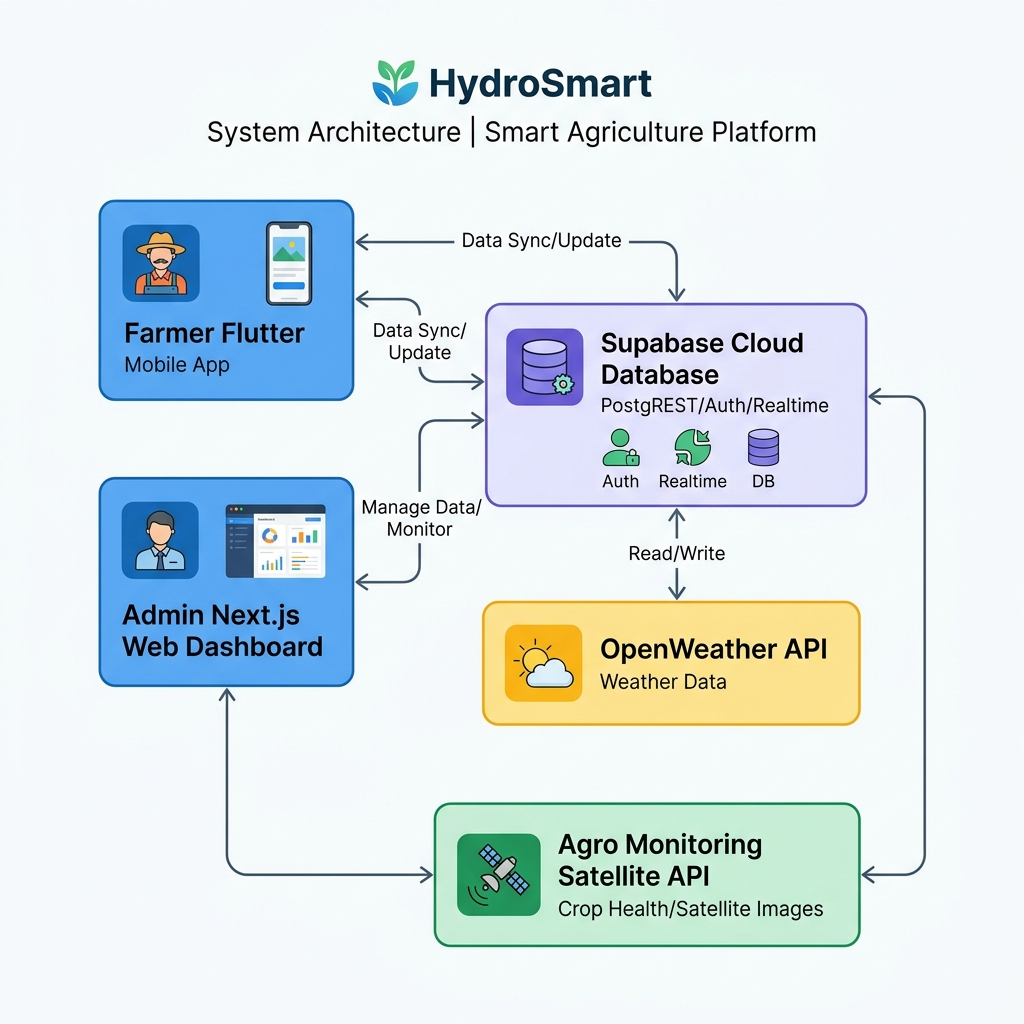
\includegraphics[width=0.9\textwidth]{architecture.png}
\caption{System Architecture of HydroSmart-MA, detailing the interactions between the Next.js backend, Flutter mobile app, Supabase database, and external weather/satellite APIs.}
\label{fig:architecture}
\end{figure>

\subsection{Software Architecture}
The backend and data layer are built on top of Next.js and Supabase (PostgreSQL). The database schema consists of several interconnected tables:
\begin{itemize}
    \item \textbf{\texttt{farmers}}: Profiles of registered users, containing regional classifications and contact information.
    \item \textbf{\texttt{plots}}: Represents agricultural fields, storing surface area (hectares), location (latitude and longitude), soil type, and crop association.
    \item \textbf{\texttt{crops}}: Stores static crop profiles including default $K_c$ values for initial, mid, and late stages, and average root depths.
    \item \textbf{\texttt{weather\_data}}: Caches local meteorological records to prevent redundant API queries.
    \item \textbf{\texttt{irrigation\_recommendations}}: Stores computed outputs, including $ET_0$, $ET_c$, net need, volume, recommended duration, and frequency.
    \item \textbf{\texttt{irrigation\_history}}: Captures actual farmer watering events for audit logging and analytics.
\end{itemize}

The Flutter mobile application communicates with the Next.js API routes via HTTP REST services. To display spatial data, the dashboard utilizes \texttt{react-leaflet} (integrating OpenStreetMap), and the mobile app uses the \texttt{flutter\_map} library, allowing farmers to physically draw or select their plots.

\subsection{Software Functionalities}
The primary software routines include:
\begin{enumerate}
    \item \textbf{Interactive Plot Creation:} Farmers select their crop and soil type, and drop a pin on the map.
    \item \textbf{Real-Time Weather Proxy:} The system queries OpenWeather API using the plot coordinates, returning temperature, relative humidity, wind speed, solar radiation, and rain.
    \item \textbf{Automated Satellite Polygon Registration:} The backend dynamically calculates a 1-hectare bounding box around the plot coordinate and registers a polygon on the Agro Monitoring API.
    \item \textbf{Evapotranspiration Core:} Computes Penman-Monteith values on the fly.
    \item \textbf{Satellite NDVI and Soil Moisture Extraction:} Queries the registered polygon to retrieve the latest Sentinel-2 NDVI average and radar-estimated volumetric soil moisture.
    \item \textbf{Admin Monitoring Dashboard:} Aggregates regional irrigation metrics, water savings indices, and historical logs.
\end{enumerate}

\section{Core Mathematical Models}

The decision engine uses FAO-56 physical formulations to model atmospheric demand, crop physiology, and soil water limits.

\subsection{Penman-Monteith Evapotranspiration ($ET_0$)}
The daily atmospheric water demand (mm/day) is modeled via:
\begin{equation}
ET_0 = \frac{0.408 \Delta (R_n - G) + \gamma \frac{900}{T + 273} u_2 (e_s - e_a)}{\Delta + \gamma (1 + 0.34 u_2)}
\end{equation}
Where:
\begin{itemize}
    \item $\Delta = \frac{4098 \cdot [0.6108 \exp(\frac{17.27 T}{T + 237.3})]}{(T + 237.3)^2}$ is the slope of the saturation vapor pressure curve ($\text{kPa}/^\circ\text{C}$).
    \item $R_n$ is net radiation (MJ/$\text{m}^2$/day), estimated from solar radiation.
    \item $G$ is the soil heat flux density (assumed $0$ for daily averages).
    \item $u_2$ is the wind speed at a 2-meter height (m/s).
    \item $e_s - e_a$ is the vapor pressure deficit (kPa), where $e_s$ is saturation vapor pressure and $e_a = e_s \times (\text{Humidity} / 100)$ is the actual vapor pressure.
    \item $\gamma = 0.665 \times 10^{-3} \times P$ is the psychrometric constant, with atmospheric pressure $P$ calculated from altitude.
\end{itemize}

\subsection{Dynamic $K_c$ from Satellite NDVI}
Traditional models use static $K_c$ curves, which assume ideal crop development. HydroSmart-MA computes the actual $K_c$ using live satellite NDVI:
\begin{equation}
K_c = 1.25 \times \text{NDVI} + 0.2
\end{equation}
subject to $0.15 \le K_c \le 1.25$. This ensures the $K_c$ reflects actual vegetative health, density, and growth speed. If satellite data is temporarily unavailable, the engine falls back to default FAO-56 lookup values for the crop.

\subsection{Daily Soil Water Balance Model}
When satellite-radar soil moisture ($SM$, $\text{m}^3/\text{m}^3$) is fetched, the root zone depletion $D_r$ (mm) is computed:
\begin{equation}
D_r = \max(1000 \cdot (FC - SM) \cdot Z_r, 0)
\end{equation}
where $FC$ is the soil field capacity (e.g., 0.38 for clay, 0.12 for sand), and $Z_r$ is the active root depth (meters). 

The software retrieves the critical depletion threshold $RAW$ (Readily Available Water):
\begin{equation}
TAW = 1000 \cdot (FC - PWP) \cdot Z_r
\end{equation}
\begin{equation}
RAW = p \cdot TAW
\end{equation}
where $PWP$ is the permanent wilting point and $p$ is the depletion fraction (commonly 0.4 to 0.5). If $D_r \ge RAW$, the soil has dried past the comfort zone of the plant, and the net irrigation need ($I_{net}$, mm) is recommended:
\begin{equation}
I_{net} = \max(D_r - \text{Rainfall}, 0)
\end{equation}
Otherwise, $I_{net} = 0$, and no irrigation is triggered. The gross water requirement is $I_{gross} = I_{net} / \eta$, where $\eta$ is the dynamic irrigation efficiency based on the soil/irrigation type (e.g. 0.90 for drip in sandy soils).

\begin{figure}[h!]
\centering
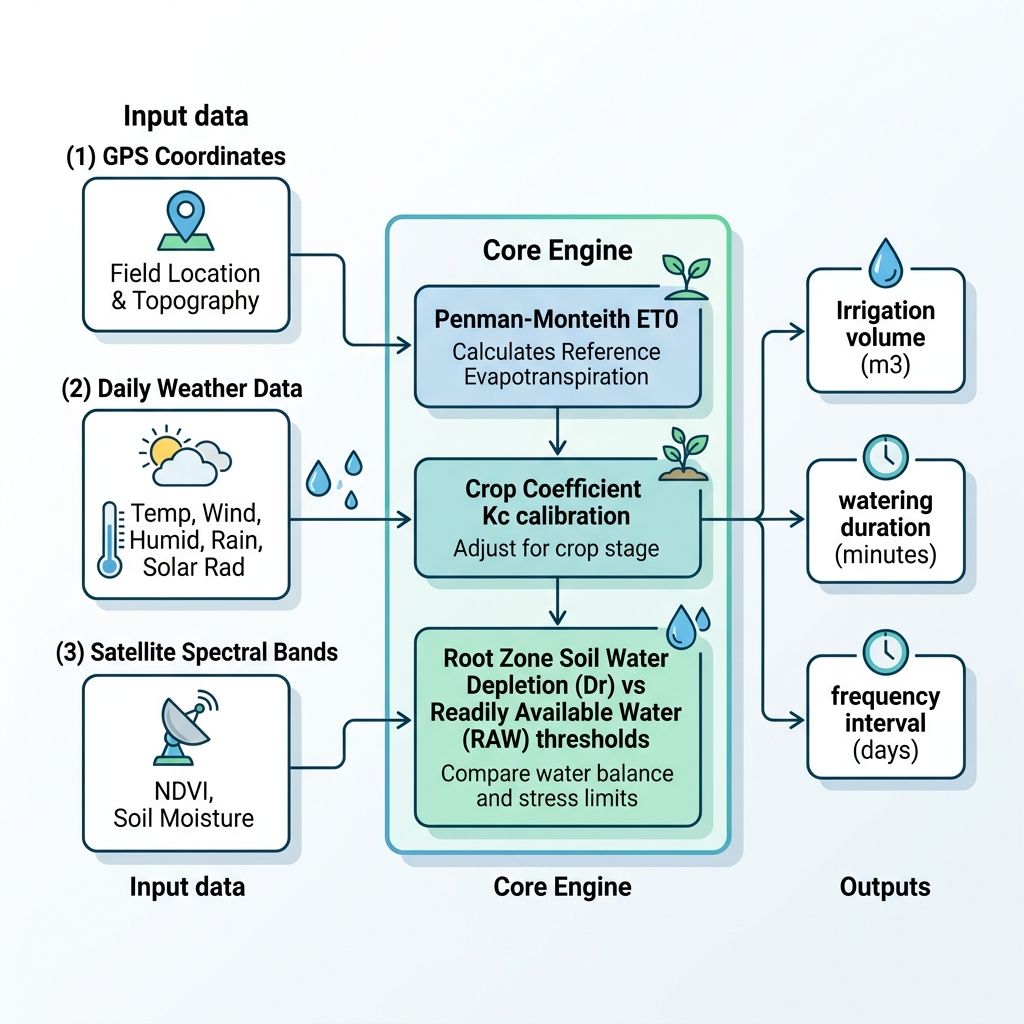
\includegraphics[width=\columnwidth]{pipeline.png}
\caption{Decision support data pipeline, illustrating weather and satellite data ingestion, crop/soil calculations, and recommendation outputs.}
\label{fig:pipeline}
\end{figure}

\section{Illustrative Scenarios and Validation}

To validate the model, we present two typical scenarios simulated in the Souss-Massa region.

\subsection{Scenario A: Sandy Drip-Irrigated Tomato Field (Summer)}
\begin{itemize}
    \item \textbf{Plot Data:} Area = 1.5 ha, Soil = sandy loam ($FC = 0.18, PWP = 0.08, \eta = 0.88$). Crop = Tomato ($Z_r = 0.6$ m, $p = 0.4$).
    \item \textbf{Weather:} High temperature, $ET_0 = 6.1$ mm/day, Rainfall = 0 mm.
    \item \textbf{Satellite:} NDVI = 0.72, yielding $K_c = 1.25 \times 0.72 + 0.2 = 1.10$. $ET_c = 6.71$ mm/day. Volumetric soil moisture $SM = 0.11$.
    \item \textbf{Calculation:}
        \begin{itemize}
            \item $TAW = 1000 \times (0.18 - 0.08) \times 0.6 = 60.0$ mm
            \item $RAW = 0.4 \times 60.0 = 24.0$ mm
            \item $D_r = 1000 \times (0.18 - 0.11) \times 0.6 = 42.0$ mm
        \end{itemize}
    \item \textbf{Decision:} Since $D_r = 42.0\text{ mm} > RAW = 24.0\text{ mm}$, irrigation is triggered. Gross irrigation need is $42.0 / 0.88 = 47.7$ mm. For a 1.5 ha plot, the recommended volume is $715.9 \text{ m}^3$. With a standard drip flow rate of 4 mm/h, the system recommends a watering duration of 11.9 hours, split over 2 days.
\end{itemize}

\subsection{Scenario B: Loamy Rainfed Olive Orchard (Winter)}
\begin{itemize}
    \item \textbf{Plot Data:} Area = 3.0 ha, Soil = loamy ($FC = 0.27, PWP = 0.12, \eta = 0.85$). Crop = Olive ($Z_r = 1.0$ m, $p = 0.5$).
    \item \textbf{Weather:} Cool temperature, $ET_0 = 2.1$ mm/day, Rainfall = 8.0 mm.
    \item \textbf{Satellite:} NDVI = 0.52, yielding $K_c = 1.25 \times 0.52 + 0.2 = 0.85$. $ET_c = 1.78$ mm/day. Soil moisture $SM = 0.24$.
    \item \textbf{Calculation:}
        \begin{itemize}
            \item $TAW = 1000 \times (0.27 - 0.12) \times 1.0 = 150.0$ mm
            \item $RAW = 0.5 \times 150.0 = 75.0$ mm
            \item $D_r = 1000 \times (0.27 - 0.24) \times 1.0 = 30.0$ mm
        \end{itemize}
    \item \textbf{Decision:} Since $D_r = 30.0\text{ mm} < RAW = 75.0\text{ mm}$, the soil water reserve is sufficient. Furthermore, the 8.0 mm of rainfall exceeds the daily crop need. The system outputs `shouldIrrigate = false`, saving $3.0\text{ ha} \times 35.3\text{ mm} \times 10 = 1059 \text{ m}^3$ of water compared to traditional daily watering practices.
\end{itemize}

\section{Impact, Reusability and Educational Value}
HydroSmart-MA's impact is threefold:
\begin{enumerate}
    \item \textbf{Agricultural & Economic Impact:} By using scientific calculations instead of guessing, smallholders can achieve water savings of 15--20\%, which directly lowers groundwater extraction energy costs (diesel/solar pumping) and preserves aquifers.
    \item \textbf{Reusability:} The software is built on modern, easily deployable technologies (Docker, Next.js, Flutter). The API endpoint `/api/recommendations` is stateless and can be consumed by external agricultural clients or third-party IoT controllers.
    \item \textbf{Educational Value:} The project serves as an open template for engineering and agronomy students in Morocco to learn how Web/Mobile technologies, GIS shapefiles, and remote sensing (Sentinel-2) intersect in modern digital agriculture.
\end{enumerate}

\section{Conclusions and Future Work}
HydroSmart-MA successfully demonstrates that satellite remote sensing and public meteorological data can be combined to build zero-hardware precision irrigation systems. Future developments will focus on integrating machine learning models (e.g. LSTM networks) to forecast soil water depletion three days in advance, allowing farmers to optimize pumping schedules based on dynamic electricity tariffs.

\section*{Acknowledgements}
We acknowledge the support of the regional agricultural development offices of Souss-Massa, Morocco, for providing the field ground truth datasets.

\end{document}
